%  Copyright 2020-2026 Robert Bosch GmbH
%
%  Licensed under the Apache License, Version 2.0 (the "License");
%  you may not use this file except in compliance with the License.
%  You may obtain a copy of the License at
%
%      http://www.apache.org/licenses/LICENSE-2.0
%
%  Unless required by applicable law or agreed to in writing, software
%  distributed under the License is distributed on an "AS IS" BASIS,
%  WITHOUT WARRANTIES OR CONDITIONS OF ANY KIND, either express or implied.
%  See the License for the specific language governing permissions and
%  limitations under the License.

\section{Installation}
Due to licensing restrictions, GitHub Copilot Extension cannot be pre-installed
in the \textbf{Robot Framework AIO} package.

You need to install it manually by executing the provided script as the
instruction in the post-installation of RobotFramework AIO setup as follows:

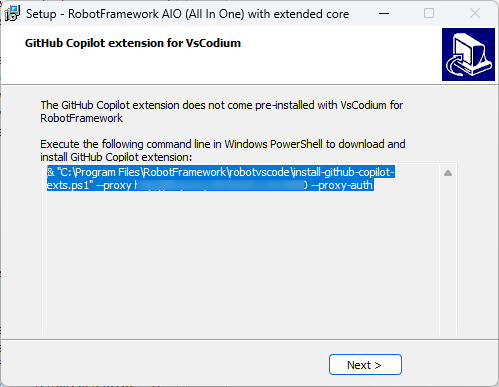
\includegraphics[width=0.5\textwidth]{./include/graphics/copilot/aio_post_installation_windows.png}

In case you missed above instruction during the setup, you can still install
the GitHub Copilot extension later by following these steps:

Open a terminal (\textbf{Windows Powershell} for Windows or Linux Terminal)
and run the appropriate script to install the GitHub Copilot extension in your
\textbf{VSCodium For RobotFramework}.
\begin{itemize}
   \item Windows Powershell:
\begin{pythonlog}
& "$env:RobotVsCode\install-github-copilot-exts.ps1" --proxy <\textless{}>your-proxy-address:port<\textgreater{}> --proxy-auth
\end{pythonlog}
   \item Linux Terminal:
\begin{pythonlog}
$RobotVsCode/install-github-copilot-exts.sh --proxy <\textless{}>your-proxy-address:port<\textgreater{}> --proxy-auth
\end{pythonlog}
\end{itemize}

The installation script will download and install the GitHub Copilot extension
in your \textbf{VSCodium For RobotFramework} environment as below:

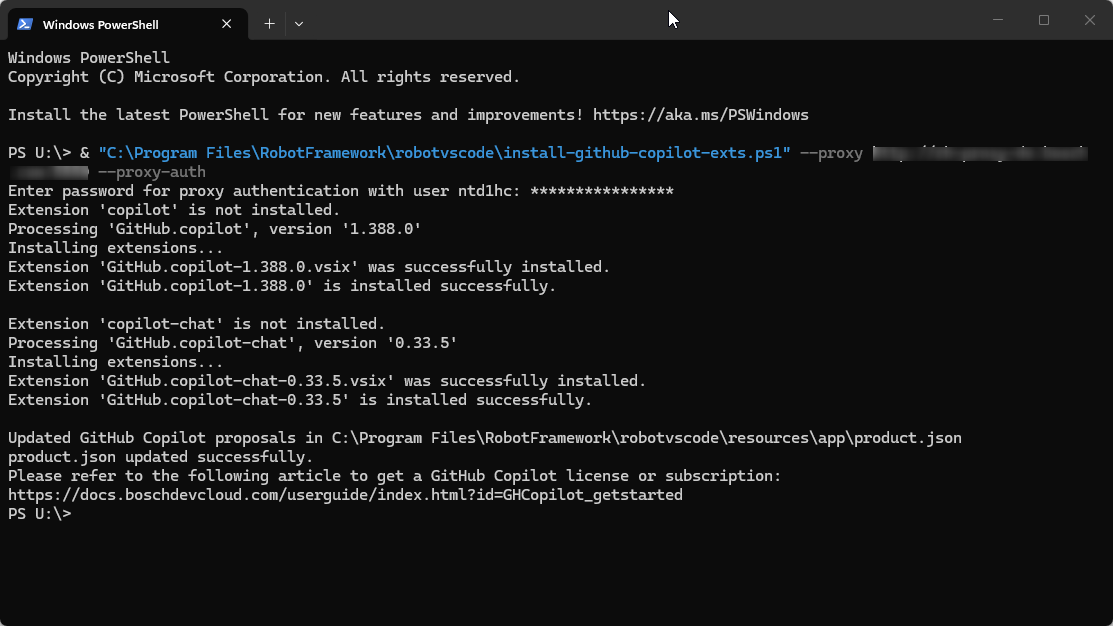
\includegraphics[width=0.9\textwidth]{./include/graphics/copilot/installation_windows.png}